To perform the computations at Site~1, namely the acquisition of the dough dataset and the collection of volume measurements, the \textbf{NVIDIA Jetson Nano Developer Kit 2GB} \cite{nvidia_corporation_jetson_nodate} was adopted.

This hardware platform is an embedded computing board designed for edge artificial intelligence applications. The device is developed by NVIDIA and belongs to the Jetson family of embedded systems specifically tailored for GPU-accelerated workloads.

The Jetson Nano 2GB is based on the NVIDIA Tegra X1 System-on-Chip (SoC), which integrates a quad-core ARM Cortex-A57 64-bit CPU and a 128-core Maxwell GPU capable of delivering up to 472 GFLOPS of FP16 compute performance. The board is equipped with 2GB of 64-bit LPDDR4 memory, which is \textbf{shared between CPU and GPU}, enabling efficient execution of deep learning inference workloads under constrained memory conditions \cite{moe_long_nvidia_nodate}.

From a hardware perspective, the development kit provides several connectivity and expansion interfaces, as shown in Figure~\ref{fig:jetson_connectivity}.

\begin{figure}[h]
    \centering
    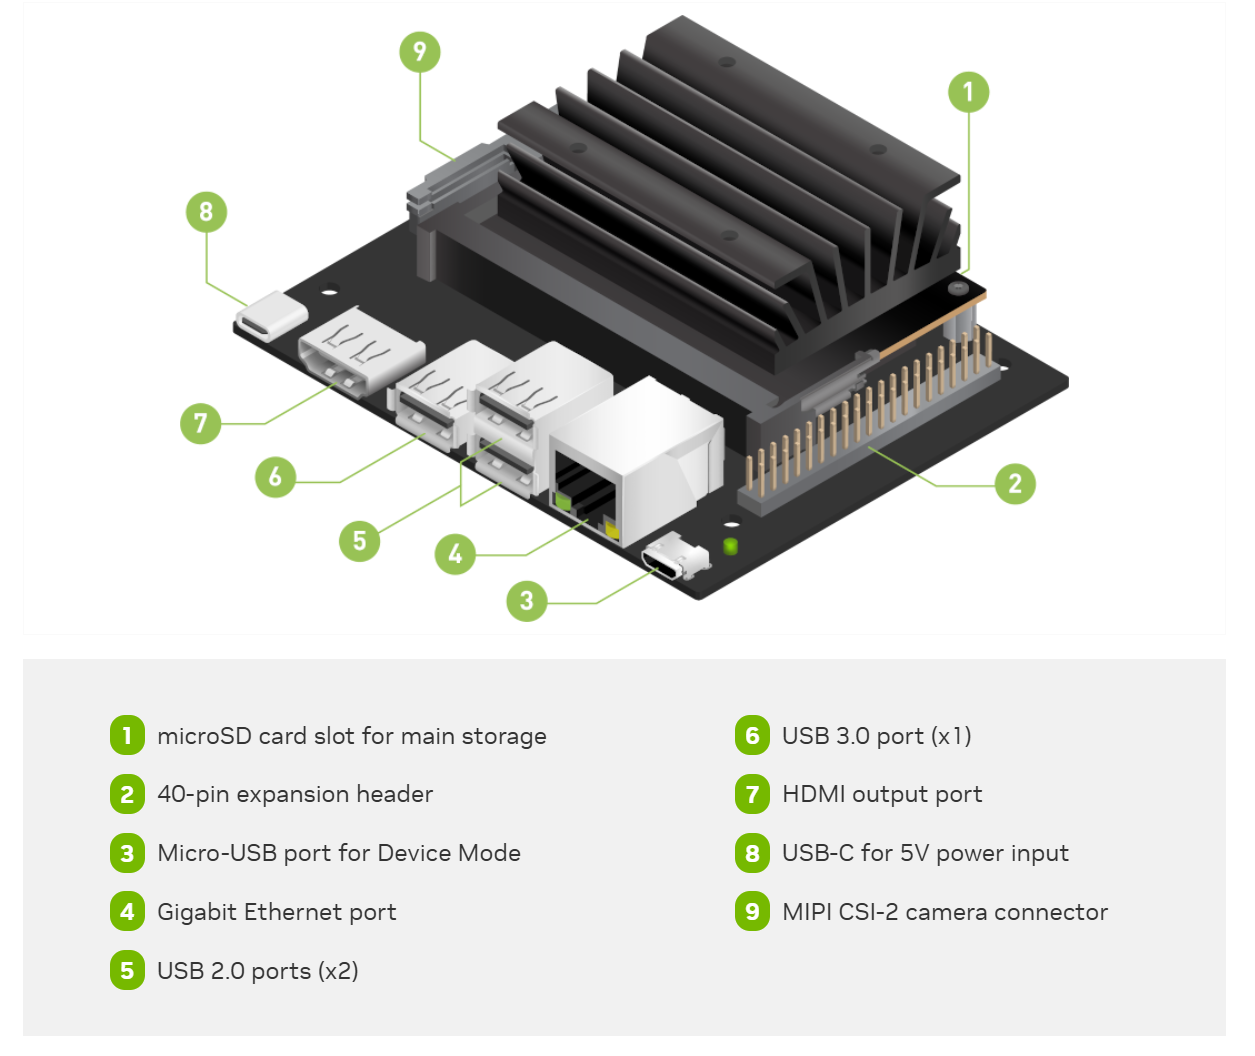
\includegraphics[width=0.4\linewidth]{images/Jetson1.png}
    \caption{NVIDIA Jetson Nano 2GB Developer Kit connectivity.}
    \label{fig:jetson_connectivity}
\end{figure}

The board operates within a typical power envelope of 5W to 10W, making it suitable for energy-constrained embedded and edge-computing scenarios. \\
The platform supports the NVIDIA JetPack SDK, which includes optimized libraries such as CUDA, cuDNN, and TensorRT for hardware-accelerated deep learning inference \cite{nvidia_corporation_jetson_nodate}.
\\
The presence of a dedicated GPU enables on-device execution of convolutional neural networks for tasks such as object detection and image segmentation, reducing latency compared to cloud-based solutions and enabling near real-time inference in edge environments. 

Despite its limited memory capacity (2GB LPDDR4) and constrained power budget, the Maxwell GPU architecture allows the Jetson Nano to achieve competitive inference performance for several state-of-the-art deep learning models. To quantitatively assess its computational capabilities, representative inference benchmarks are reported in Table~\ref{tab:jetson_benchmarks} \cite{moe_long_nvidia_nodate}. The values are expressed in frames per second (FPS) under optimized inference configurations.

\begin{table}[h]
\centering
\begin{tabular}{l c}
\hline
\textbf{Model} & \textbf{Performance (FPS)} \\
\hline
Inception-v4 & 10.51 \\
VGG-19 & 9.95 \\
Super-resolution (BSD500) & 15.12 \\
U-Net (segmentation) & 16.57 \\
Pose estimation & 14.47 \\
YOLOv3-Tiny (416$\times$416) & 47.11 \\
ResNet-50 (224$\times$224) & 36.42 \\
SSD MobileNet-v1 & 42.00 \\
\hline
\end{tabular}
\caption{Representative inference performance of NVIDIA Jetson Nano 2GB.}
\label{tab:jetson_benchmarks}
\end{table}

As shown in Table~\ref{tab:jetson_benchmarks} \cite{moe_long_nvidia_nodate}, lightweight architectures such as YOLOv3-Tiny and SSD MobileNet-v1 achieve real-time performance, while more computationally demanding networks (e.g., VGG-19 and Inception-v4) operate at lower frame rates. These results highlight the importance of selecting architectures that balance accuracy and computational complexity when deploying deep learning models on resource-constrained embedded platforms.
\\
It should be noted that the reported performance values may vary depending on the software configuration, precision mode (e.g., FP16 or INT8), and system workload.


Considering the trade-off between computational performance, power consumption, cost, and ecosystem support, the Jetson Nano 2GB represents a suitable platform for prototyping and deploying computer vision algorithms in embedded systems, as in the present application.